
\subsubsection{フロアマップを用いた歩行可能座標への補正}

% TODO:ここのフォーマットの統一
図\ref{fig:pdr-rotate}に示した軌跡には人間が歩行可能座標ではない場所を
通過している問題ある.図\ref{fig:walkable-points}は
軌跡上の点が歩行可能な座標であるか否かを示している.青色の点は
歩行可能な座標上に存在する点を,赤色の点は歩行不可能な座標上に
存在する点を表している.この図から分かるように軌跡の一部が壁や
障害物の存在する座標を通過している.このような軌跡は人間の実際の
歩行経路としては物理的に不適切である.
この問題に対してフロアマップ情報を用いた歩行不可能座標の補正機能を実装している.
この機能は節3.2.2.3で説明したフロアマップ情報を利用し,MapMatchCorrectorクラスの一機能として提供している.



% TODO 2.前の項で出したマップマッチングとの関係性についても触れてもいいのかもしれない,
% こちらはより詳細なマップマッチングな気がする?

\begin{figure}[H]
    \centering
    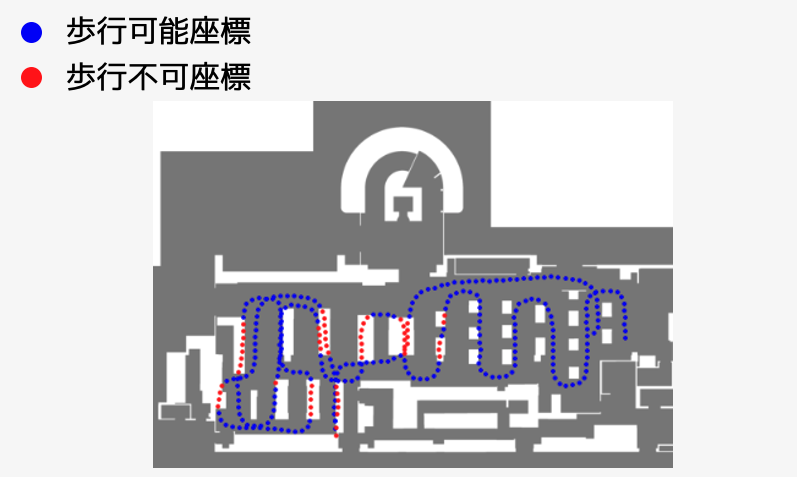
\includegraphics[width=\linewidth]{../image/unwalkable_points.jpg}
    \caption{
      軌跡上の歩行可能座標と歩行不可能座標の可視化
    }    \label{fig:unwalkable_points}
\end{figure}


補正処理は以下の手順で行われる.まず軌跡上の各点について,
その座標がフロアマップ上の歩行可能座標に存在するかを判定する.
ある時刻$t$の座標$(x_t, y_t)$が歩行不可能な座標に存在する場合,
その点からもっとも近い歩行可能な座標$(x_t^*, y_t^*)$を探索する.
この探索には幅優先探索(BFS)アルゴリズムを用いる.
BFSは最短経路を保証し探索範囲を同心円状に広げていくため,
もっとも近い歩行可能座標を確実に発見できる.
またフロアマップのような格子状の探索空間では,
探索の実装が単純かつ効率的な利点を持つ.
具体的には現在の座標から上下左右および斜め方向に探索を行い,
最初に見つかった歩行可能な座標を $(x_t^*, y_t^*)$ として採用する.
この際探索はフロアマップを表現する行列の範囲を超えないように制限される.
歩行可能な座標が見つかった場合時刻$t$以降の全ての軌跡の座標を,
式\eqref{eq:move}に従って平行移動する.
ここで$(x_k', y_k')$は補正後の座標,$(x_k, y_k)$は補正前の座標を表す.
またこの補正処理は軌跡の始点から順に適用される.% TODO:ここにこの文あるの違和感がある.
この処理により歩行不可能座標に存在していた点とそれ以降の軌跡が,
もっとも近い歩行可能な座標へと移動される.
図\ref{fig:walkable-points}に示すように,補正後の軌跡では全ての点が歩行可能な座標内に存在している.
なおこの補正処理は前節までの補正とは異なり,軌跡の進行方向は保持したまま位置のみを補正する特徴がある.


\begin{equation}
  \label{eq:move}
x_k' = x_k + (x_t^* - x_t), \quad y_k' = y_k + (y_t^* - y_t) \quad (k \geq t)
\end{equation}


% TODO:2.この処理をしても壁抜けは防げないのを説明した方がいいかもしれない
\begin{figure}[H]
    \centering
    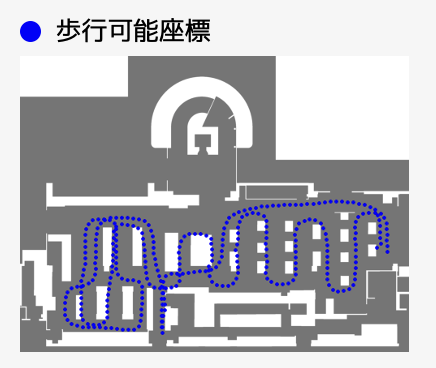
\includegraphics[width=\linewidth]{../image/walkable-points.jpg}
    \caption{歩行可能座標への補正適用後の軌跡}    \label{fig:walkable-points}
\end{figure}
